\chapter{Arbeid og energi}
\intro{Arbeid og energi er to grunnleggende begreper i fysikk som hjelper oss å forstå hvordan krefter påvirker objekter, og hvordan energi overføres eller omdannes i ulike systemer. Når en kraft virker på et objekt og forårsaker en forflytning, sier vi at det er utført et arbeid. Dette arbeidet resulterer ofte i en endring av objektets energi, enten som bevegelsesenergi (kinetisk energi) eller som lagret energi (potensiell energi). Energi kan ikke forsvinne; den kan bare overføres eller omdannes fra én form til en annen. Dette er kjent som energiens bevaringslov, som er en av de mest fundamentale prinsippene i fysikk. }

\spm{}{%
Hva er arbeid i fysisk forstand?\\
Hva er energi, og i hvilke former finnes den?\\
Hva sier energibevaringsloven?}
\newpage

\section{Arbeid}
I fysikk utfører vi arbeid når en kraft flytter et objekt over en avstand. Når en kraft \( \vec{F} \) virker på et objekt og forårsaker en forflytning \( \vec{s} \), utføres det et arbeid dersom kraften og forflytningen ikke er vinkelrette på hverandre. Arbeidet er størst når kraften virker i samme retning som forflytningen, og null når kraften virker vinkelrett på forflytningen.

\defn{Arbeid}{
    Matematisk kan arbeid \( W \) uttrykkes som:
    \begin{align}
        W = \vec{F} \cdot \vec{s} = F \cdot s \cdot \cos(\theta)
    \end{align}
    hvor \( \vec{F} \) er kraftvektoren, \( \vec{s} \) er forflytningsvektoren, og \( \theta \) er vinkelen mellom kraften og forflytningen. Dersom \( \theta = 0^\circ \), er \( \cos(\theta) = 1 \), og arbeidet er maksimalt. Arbeid måles i joule (J), som tilsvarer newtonmeter (N·m).
}

\exm{Dytte en boks}{
    Tenk deg at du dytter en boks langs et gulv med en kraft på \( 10 \, \text{N} \) over en avstand på \( 5 \, \text{m} \). Kraften du bruker er i samme retning som bevegelsen (\( \theta = 0^\circ \)). Da kan vi regne ut arbeidet slik:
    \[
    W = F \cdot d \cdot \cos(\theta) = 10 \, \text{N} \cdot 5 \, \text{m} \cdot \cos(0^\circ)
    \]
    \[
    W = 10 \, \text{N} \cdot 5 \, \text{m} \cdot 1 = 50 \, \text{J}
    \]
    Arbeidet som utføres er \( 50 \, \text{J} \).
}

\begin{figure}[ht!]
    \centering
    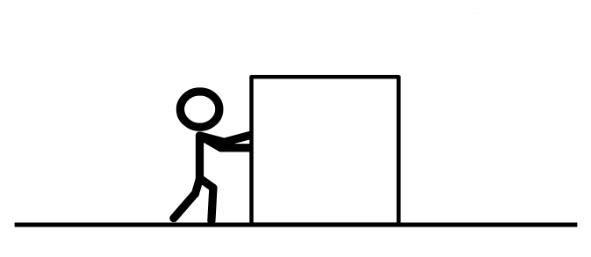
\includegraphics[width=0.8\textwidth]{Images/Kapittel3:Arbeid&Energi/Arbeidbokseksempel.png}
    \caption{Dytte en boks}
    \label{fig:Dytte_en_boks}
    \end{figure}

\tips{Husk vinkelen}{
    Når du beregner arbeid, er det viktig å ta hensyn til vinkelen \( \theta \) mellom kraften og forflytningen. Hvis vinkelen er 90 grader, blir det ikke utført noe arbeid, selv om en kraft er til stede. Hvis vinkelen er 0 grader, er arbeidet maksimalt, fordi all kraften virker i forflytningens retning.
}

\defn{Arbeid for å presse sammen en fjær}{
    Når en fjær presses sammen eller strekkes, utføres et arbeid som lagrer energi i fjæren som elastisk potensiell energi. Denne typen arbeid kan uttrykkes ved hjelp av Hookes lov, som sier at kraften \( F \) som virker på fjæren er proporsjonal med forlengelsen eller sammentrekningen \( x \) av fjæren:
    \[
    F = k \cdot x
    \]
    hvor \( k \) er fjærkonstanten som måler fjærens stivhet. For å presse sammen en fjær fra en posisjon \( x = 0 \) til \( x = x \), kan arbeidet \( W \) beregnes som:
    \begin{align}
        W = \frac{1}{2} k x^2
    \end{align}
    Dette viser at arbeidet som utføres for å komprimere fjæren er proporsjonalt med kvadratet av fjærens forskyvning. Den energien som lagres i fjæren som et resultat av dette arbeidet kalles elastisk potensiell energi, og måles i joule (J).
}

\noindent % Dette sørger for at det ikke er noe innrykk
\begin{minipage}{0.45\textwidth}
    \centering
    \raisebox{5mm}{ % Løfter bildet litt opp, juster verdien etter behov
        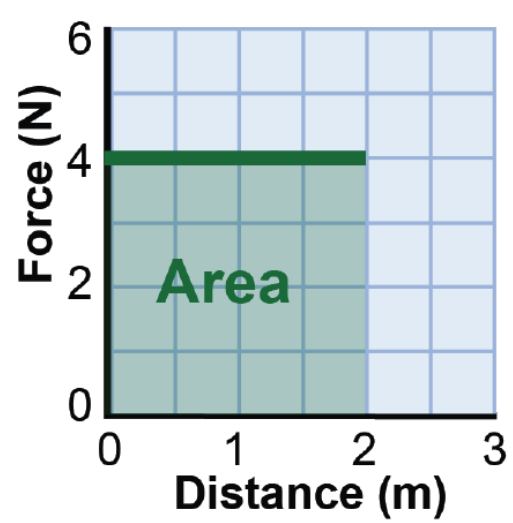
\includegraphics[width=\linewidth]{Images/Kapittel3:Arbeid&Energi/Arbeidpåboksgraf.png}
    }
    \captionof{figure}{Arealet er eksempel på arbeidet på en boks, \( W = F \cdot s \).}
    \label{fig:image1}
\end{minipage}\hfill
\begin{minipage}{0.45\textwidth}
    \centering
    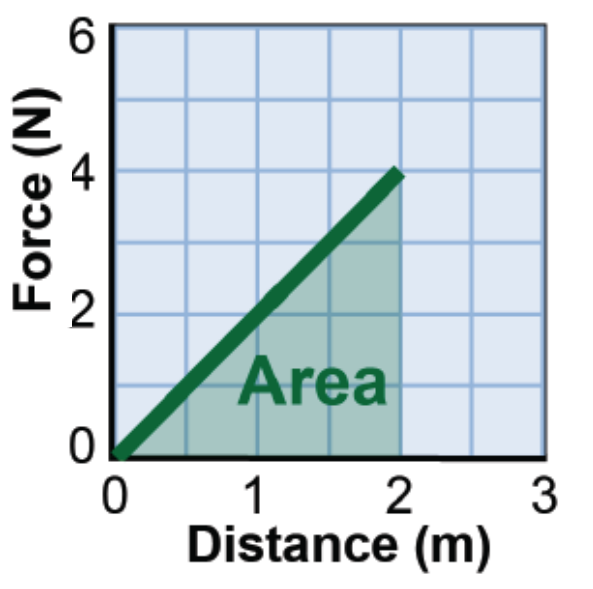
\includegraphics[width=\linewidth]{Images/Kapittel2:Kinematikk/Arbeidpåfjærgraf.png}
    \captionof{figure}{Arealet er eksempel på arbeidet for å presse sammen en fjær, når \( F = k \cdot x \) og \( W = \frac{1}{2} k x^2 \).}
    \label{fig:image2}
\end{minipage}

\section{Energi}

I fysikk beskriver energi et legemes evne til å påvirke omgivelsene, enten ved å utføre arbeid eller overføre varme. Når en kraft virker på et objekt og forårsaker en forflytning, blir energi overført til objektet gjennom arbeidet som utføres. Derfor kan arbeid sees som en måte å overføre energi på mellom objekter eller systemer.

Det finnes mange ulike former for energi, som kinetisk energi (bevegelsesenergi) og potensiell energi (lagret energi). Disse formene gir objekter mulighet til å påvirke andre objekter eller endre deres tilstand, for eksempel ved å flytte dem, deformere dem, eller varme dem opp. Arbeid og energi måles begge i joule (J), som er standardenheten for energi i fysikk.

Ifølge energibevaringsloven kan energi verken skapes eller ødelegges, kun omformes fra en form til en annen. 

\subsection{Kinetisk energi}

Tenk deg at en bil kjører nedover en vei. Bilen har kinetisk energi på grunn av sin bevegelse. Kinetisk energi er den energien et objekt har fordi det er i bevegelse. Jo raskere objektet beveger seg, desto mer kinetisk energi har det. For en bil vil både massen \( m \) og hastigheten \( v \) påvirke hvor mye kinetisk energi den har.

\defn{Kinetisk Energi}{
    Matematisk kan den kinetiske energien \( E_k \) uttrykkes som:
    \begin{align}
        E_k = \frac{1}{2} m v^2
    \end{align}
    hvor \( m \) er massen til objektet og \( v \) er hastigheten.
}

Kinetisk energi er en viktig form for energi, som spiller en sentral rolle i mange fysiske prosesser som kollisjoner, bevegelse og energioverføringer. Når bilen bremser ned og stopper, reduseres dens kinetiske energi til null fordi hastigheten \( v \) også blir null.

\begin{figure}[ht!]
    \centering
    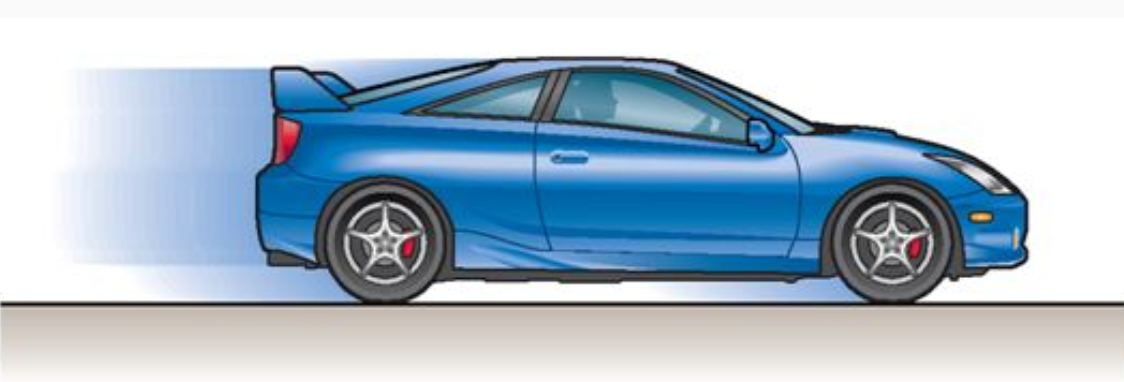
\includegraphics[width=0.8\textwidth]{Images/Kapittel3:Arbeid&Energi/Bil_kinetisk.png}
    \caption{Kinetisk energi i kjørende bil}
    \label{fig:Dytte_en_boks}
    \end{figure}

\defn{Arbeid og endring i kinetisk energi}{
    Arbeid-energi-teoremet sier at arbeidet \( W \) som utføres på et objekt er lik endringen i objektets kinetiske energi:
    \[
    W = \Delta E_k = E_k^{\text{slutt}} - E_k^{\text{start}}
    \]
    For å se dette, starter vi med definisjonen av arbeid som kraft ganget med forflytning:
    \[
    W = F \cdot s
    \]
    I følge Newtons andre lov er \( F = m \cdot a \), der \( a \) er akselerasjonen. Arbeid kan dermed skrives som:
    \[
    W = m \cdot a \cdot s
    \]
    Ved å bruke bevegelseslikningen \( v^2 = v_0^2 + 2as \), som beskriver forholdet mellom hastighet, akselerasjon og forflytning, kan vi erstatte \( a \cdot d \) med \( \frac{v^2 - v_0^2}{2} \). Dermed blir arbeidet:
    \[
    W = m \cdot \frac{v^2 - v_0^2}{2}
    \]
    Dette viser at arbeidet utført på objektet er lik endringen i dets kinetiske energi:
    \[
    W = \Delta E_k = \frac{1}{2} m v^2 - \frac{1}{2} m v_0^2
    \]
}

\vspace{20pt} % Gir ekstra mellomrom på 10 punkter

\exm{Horisontal bevegelse med friksjon}{
En kloss med masse \(0.8 \, \text{kg}\) har en startfart på \(2.0 \, \text{m/s}\) og blir flyttet med en horisontal kraft på \(8.0 \, \text{N}\). Friksjonskraften som virker mot bevegelsen er \(5.6 \, \text{N}\), og etter å ha blitt flyttet \(2.0 \, \text{m}\) får klossen en fart på \(4.0 \, \text{m/s}\).

\textbf{Del 1: Endringen i kinetisk energi} \\
\textit{Metode:} Kinetisk energi \(E_k\) beregnes med formelen \(E_k = \frac{1}{2} m v^2\). Endringen i kinetisk energi \( \Delta E_k \) er forskjellen mellom slutt- og startenergien:
\[
E_k^{\text{start}} = \frac{1}{2} \cdot 0.8 \, \text{kg} \cdot (2.0 \, \text{m/s})^2 = \frac{1}{2} \cdot 0.8 \cdot 4 = 1.6 \, \text{J}
\]
\[
E_k^{\text{slutt}} = \frac{1}{2} \cdot 0.8 \, \text{kg} \cdot (4.0 \, \text{m/s})^2 = \frac{1}{2} \cdot 0.8 \cdot 16 = 6.4 \, \text{J}
\]
Endringen i kinetisk energi er:
\[
\Delta E_k = E_k^{\text{slutt}} - E_k^{\text{start}} = 6.4 \, \text{J} - 1.6 \, \text{J} = 4.8 \, \text{J}
\]

\textbf{Del 2: Arbeid utført på klossen} \\
\textit{Metode:} Arbeid \(W\) er definert som kraft ganger forflytning, men i dette tilfellet må vi ta hensyn til både den horisontale kraften og friksjonskraften som virker mot bevegelsen. Det totale arbeidet \( W \) kan beregnes som summen av arbeidet utført av begge kreftene:
\[
W_{\text{totalt}} = W_{\text{kraft}} + W_{\text{friksjon}} = F \cdot s - F_{\text{friksjon}} \cdot s
\]
Her er kraften \( F = 8.0 \, \text{N} \), friksjonskraften \( F_{\text{friksjon}} = 5.6 \, \text{N} \), og forflytningen \( d = 2.0 \, \text{m} \):
\[
W_{\text{totalt}} = 8.0 \, \text{N} \cdot 2.0 \, \text{m} - 5.6 \, \text{N} \cdot 2.0 \, \text{m} = 16.0 \, \text{J} - 11.2 \, \text{J} = 4.8 \, \text{J}
\]

}


\subsection{Potensiell energi}

Potensiell energi er energien som er lagret i et objekt på grunn av dets posisjon eller tilstand. Et vanlig eksempel på potensiell energi er gravitasjonspotensiell energi, som avhenger av et objekts høyde over bakken og tyngdekraften. Når et objekt løftes opp fra bakken, lagres det energi som potensiell energi, og denne energien kan omformes til kinetisk energi når objektet faller tilbake mot bakken.

\defn{Gravitasjonspotensiell Energi}{
    Matematisk kan gravitasjonspotensiell energi \( E_p \) uttrykkes som:
    \begin{align}
        E_p = mgh
    \end{align}
    hvor \( m \) er massen til objektet, \( g \) er tyngdeakselerasjonen (som på jorden har en verdi på \( 9.81 \, \text{m/s}^2 \)), og \( h \) er høyden over et valgt nullnivå. 
}

\begin{figure}[ht!]
    \centering
    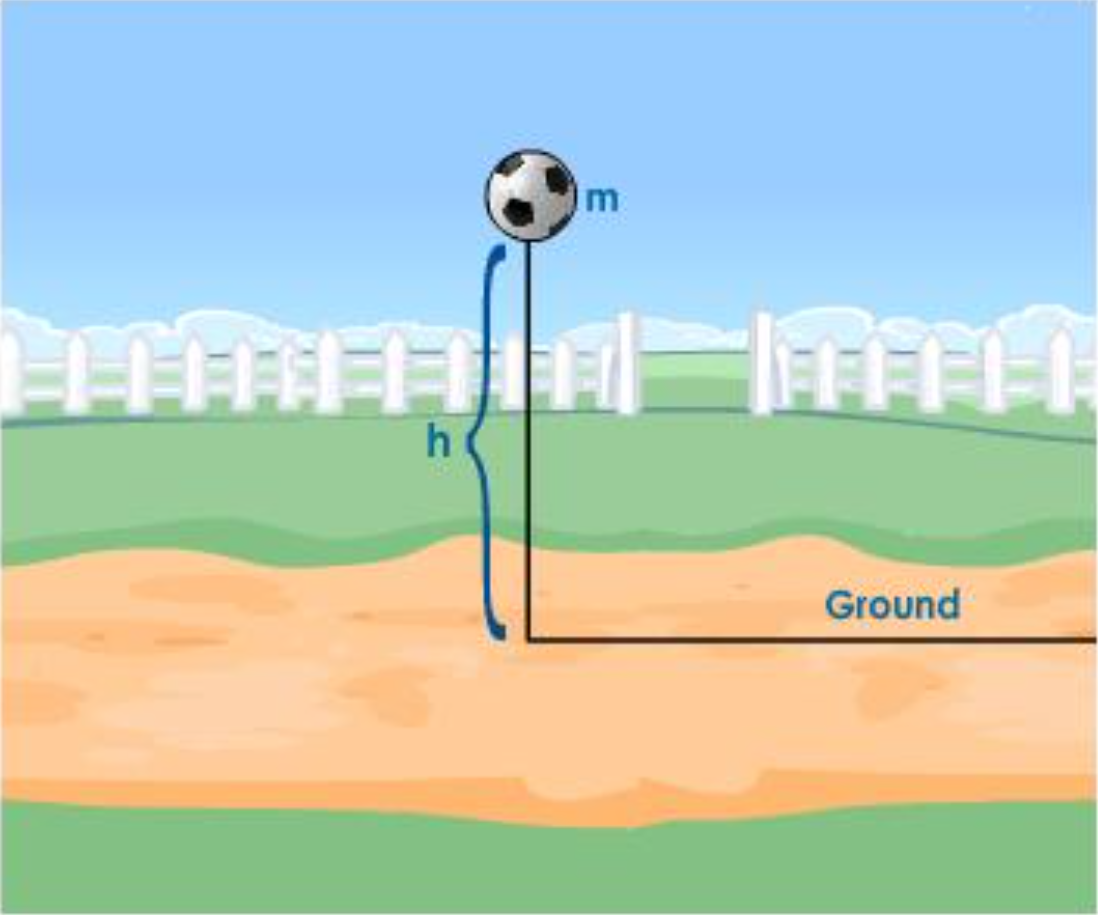
\includegraphics[width=0.6\textwidth]{Images/Kapittel3:Arbeid&Energi/Ball_over_bakken.png}
    \caption{Potensiell energi i ball med høydeavstand}
    \label{fig:Dytte_en_boks}
    \end{figure}

\defn{Utledning av Gravitasjonspotensiell Energi}{
    Arbeidet som må utføres på et legeme med masse \( m \) for å løfte det en høyde \( h \) i tyngdefeltet, er gitt ved:
    \[
    W = F \cdot h
    \]
    hvor kraften \( F \) som virker på objektet er tyngdekraften, \( F = m \cdot g \). Dermed blir arbeidet:
    \[
    W = m \cdot g \cdot h
    \]
    Dette arbeidet er lik den potensiell energien \( E_p \) som er lagret i objektet. Derfor får vi:
    \[
    E_p = m \cdot g \cdot h
    \]
}


Potensiell energi kan også finnes i andre former, som elastisk potensiell energi, som er energien lagret i en elastisk fjær når den strekkes eller presses sammen. Potensiell energi er alltid relatert til en posisjon eller en tilstand som gir objektet muligheten til å utføre arbeid når energien frigjøres.


\defn{Elastisk Potensiell Energi}{
    For en fjær kan den elastiske potensiell energien \( E_p \) uttrykkes som:
    \begin{align}
        E_p = \frac{1}{2} k x^2
    \end{align}
    hvor \( k \) er fjærkonstanten som beskriver fjærens stivhet, og \( x \) er forlengelsen eller kompresjonen fra fjærens likevektsposisjon. 
}

\begin{figure}[ht!]
    \centering
    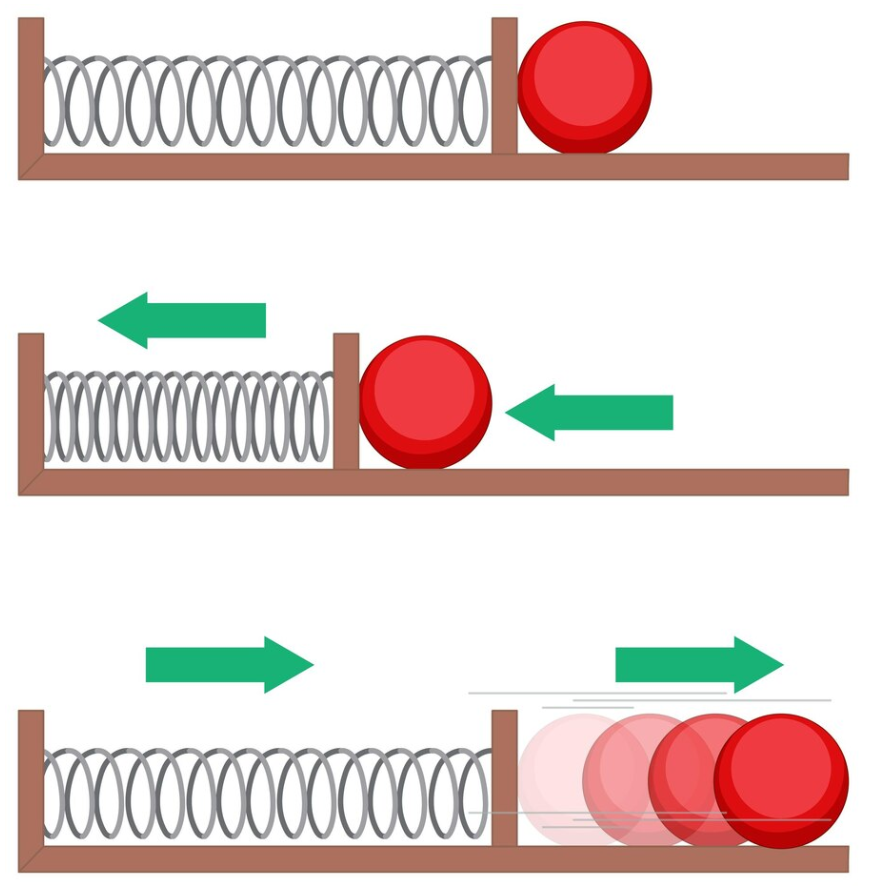
\includegraphics[width=0.4\textwidth]{Images/Kapittel3:Arbeid&Energi/fjær.png}
    \caption{Energi i ball på fjær}
    \label{fig:Dytte_en_boks}
    \end{figure}

\newpage

\section{Energitap}
Energitap skjer når energi omdannes fra en nyttig form, som kinetisk eller potensiell energi, til former som varme eller lyd. Dette skjer ofte på grunn av friksjon eller motstand i systemet. For eksempel vil et objekt som beveger seg langs en overflate oppleve friksjon, som omdanner noe av den kinetiske energien til varme. 

Selv om den totale energien i systemet bevares, reduserer energitap den mengden energi som kan brukes til arbeid. Energitap er derfor en viktig faktor i mange praktiske situasjoner, som ingeniørarbeid og fysikkproblemer.

\exm{Energiforskjell og energitap i et fall}{
En ball med masse \( 0.5 \, \text{kg} \) slippes fra en høyde på \( 10 \, \text{m} \). Rett før ballen treffer bakken, har den en hastighet på \( 12 \, \text{m/s} \). Vi antar at noe energi har gått tapt på grunn av luftmotstand. Beregn energitapet ved å sammenligne den potensielle energien på toppen med den kinetiske energien rett før bakken. \\

\textbf{Del 1: Potensiell energi på toppen} \\
Den potensielle energien ballen har på toppen, før den slippes, kan beregnes med formelen:
\[
E_p = mgh
\]
hvor \( m = 0.5 \, \text{kg} \), \( g = 9.81 \, \text{m/s}^2 \), og \( h = 10 \, \text{m} \):
\[
E_p = 0.5 \, \text{kg} \cdot 9.81 \, \text{m/s}^2 \cdot 10 \, \text{m} = 49.05 \, \text{J}
\]
Dette er den totale potensielle energien som ballen har før fallet.

\textbf{Del 2: Kinetisk energi rett før bakken} \\
Når ballen nærmer seg bakken med en hastighet på \( 12 \, \text{m/s} \), kan vi beregne dens kinetiske energi:
\[
E_k = \frac{1}{2} m v^2
\]
hvor \( m = 0.5 \, \text{kg} \) og \( v = 12 \, \text{m/s} \):
\[
E_k = \frac{1}{2} \cdot 0.5 \, \text{kg} \cdot (12 \, \text{m/s})^2 = 36 \, \text{J}
\]
Dette er den kinetiske energien ballen har rett før den treffer bakken.

\textbf{Del 3: Energitap på grunn av luftmotstand} \\
Forskjellen mellom den potensielle energien på toppen og den kinetiske energien rett før bakken gir oss energitapet som følge av luftmotstand:
\[
\Delta E = E_p - E_k = 49.05 \, \text{J} - 36 \, \text{J} = 13.05 \, \text{J}
\]
Dette betyr at \( 13.05 \, \text{J} \) av energien har blitt tapt på grunn av luftmotstanden i løpet av fallet.
}


\section{Bevaring av mekanisk energi}

I et lukket system, der det ikke er noen energitap til friksjon eller andre motstandskrefter, er den mekaniske energien bevart. Mekanisk energi er summen av et objekts kinetiske energi \( E_k \) og potensielle energi \( E_p \). Bevaringsloven sier at den totale mekaniske energien i et system forblir konstant, så lenge det ikke er energitap på grunn av motstand som friksjon eller luftmotstand.

Matematisk kan bevaring av mekanisk energi uttrykkes som:
\[
E_{\text{mekanisk}} = E_k + E_p = \text{konstant}
\]
Dette betyr at i et system der mekanisk energi er bevart, vil all potensiell energi som et objekt mister omformes til kinetisk energi, og omvendt. For eksempel, når en ball faller fra en høyde, vil dens potensielle energi omformes til kinetisk energi når den nærmer seg bakken. I fravær av luftmotstand vil den totale energien forbli den samme gjennom hele bevegelsen.

Når det oppstår friksjon eller andre energitap, vil den mekaniske energien ikke være bevart, fordi noe av energien omformes til andre former, som varme.

\defn{Bevaring av mekanisk energi}{
    Når et legme beveger seg under påvirkning av kun tyngdekraft og/ eller fjærkraft, er energien bevart og kan skrives slik:  
    \begin{align}
        E_{\text{før}} = E_{\text{etter}}
    \end{align}
    hvor den totale mekaniske energien \( E \) er summen av gravitasjonspotensiell energi, kinetisk energi og elastisk potensiell energi. Dette kan skrives som:
    \begin{align}
        E = mgh + \frac{1}{2} m v^2 + \frac{1}{2} k x^2
    \end{align}
    Her er \( m \) massen til objektet, \( g \) tyngdeakselerasjonen, \( h \) høyden over et nullnivå, \( v \) hastigheten, \( k \) fjærkonstanten, og \( x \) forlengelsen eller kompresjonen av en fjær. 
}

\exm{Fallende stein}{
En person holder en stein på en høyde \(1.60 \, \text{m}\) over bakken og slipper den. Vi skal regne ut steinens hastighet rett før den treffer bakken. Vi antar at luftmotstanden er neglisjerbar.

\textit{Metode:} \\
Når steinen slippes, har den ingen startfart, så det er ingen kinetisk energi i systemet ved start. Den har kun potensiell energi på grunn av høyden over bakken. Vi setter nullpunktet for høyden til bakkenivå, slik at høyden \( h = 0 \) rett før steinen treffer bakken. På dette tidspunktet er den potensielle energien null, og all energien er omformet til kinetisk energi.

Vi bruker bevaring av mekanisk energi, som sier at total energien før og etter fallet er den samme:
\[
E_{\text{før}} = E_{\text{etter}}
\]
I starten har steinen potensiell energi, men ingen kinetisk energi. Den totale energien i starten kan skrives som:
\[
mgh_1 + \frac{1}{2} m v_1^2 = mgh_2 + \frac{1}{2} m v_2^2
\]
Siden steinen slippes uten startfart, er hastigheten ved starten \( v_1 = 0 \), og dermed er det ingen kinetisk energi i starten:
\[
mgh_1 + \frac{1}{2} m \cdot 0^2 = mgh_2 + \frac{1}{2} m v_2^2
\]
Rett før steinen treffer bakken, er høyden \( h_2 = 0 \), og dermed er det ingen potensiell energi på dette tidspunktet:
\[
mgh_1 + 0 = 0 + \frac{1}{2} m v_2^2
\]
Vi kan nå stryke massen \( m \) fra begge sider av likningen:
\[
gh_1 = \frac{1}{2} v_2^2
\]
Løs for hastigheten \( v_2 \):
\[
v_2 = \sqrt{2gh_1}
\]
Ved å sette inn verdiene \( g = 9.8 \, \text{m/s}^2 \) og \( h_1 = 1.60 \, \text{m} \), får vi:
\[
v_2 = \sqrt{2 \cdot 9.8 \, \text{m/s}^2 \cdot 1.60 \, \text{m}} = \sqrt{31.36} \approx 5.6 \, \text{m/s}
\]
Steinen har en hastighet på \( 5.6 \, \text{m/s} \) rett før den treffer bakken.
}


\begin{figure}[ht!]
    \centering
    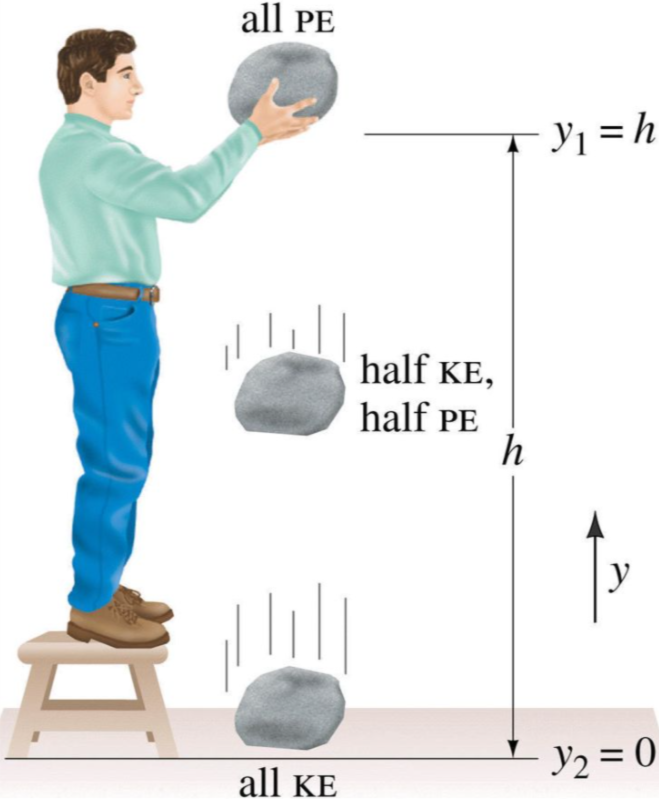
\includegraphics[width=0.4\textwidth]{Images/Kapittel3:Arbeid&Energi/Fallende stein.png}
    \caption{Fallende stein}
    \label{fig:Stein}
    \end{figure}

\exm{Fjærkanon i tyngdefeltet - Finn fjærkonstanten \( k \)}{
En fjærkanon skyter en kanonkule med masse \(0.2 \, \text{kg}\) rett opp i luften etter at fjæren har blitt komprimert med \( x = 0.15 \, \text{m} \). Kanonkulen når en maksimal høyde på \( h = 5.0 \, \text{m} \) før den faller tilbake ned igjen. Anta at all fjærens elastiske potensielle energi omformes til kanonkulas potensielle energi på toppen. Vi skal finne fjærkonstanten \( k \) for fjæren.

\textit{Metode:} \\
Vi bruker bevaring av mekanisk energi, som sier at all elastisk potensiell energi i fjæren omformes til gravitasjonspotensiell energi på toppen. Elastisk potensiell energi for fjæren er gitt ved:
\[
E_{\text{fjær}} = \frac{1}{2} k x^2
\]
Den potensielle energien kanonkulen har på toppen er:
\[
E_p = mgh
\]
Siden \( E_{\text{fjær}} = E_p \), kan vi sette opp likningen:
\[
\frac{1}{2} k x^2 = mgh
\]
Vi løser for fjærkonstanten \( k \):
\[
k = \frac{2mgh}{x^2}
\]
Nå setter vi inn verdiene \( m = 0.2 \, \text{kg} \), \( g = 9.8 \, \text{m/s}^2 \), \( h = 5.0 \, \text{m} \), og \( x = 0.15 \, \text{m} \):
\[
k = \frac{2 \cdot 0.2 \, \text{kg} \cdot 9.8 \, \text{m/s}^2 \cdot 5.0 \, \text{m}}{(0.15 \, \text{m})^2} = \frac{19.6 \, \text{N/m} \cdot \text{m}}{0.0225 \, \text{m}^2} = \doubleunderline{871.1 \, \text{N/m}}
\]
Fjærkonstanten \( k \) er dermed \( 871.1 \, \text{N/m} \).
}


\begin{figure}[ht!]
    \centering
    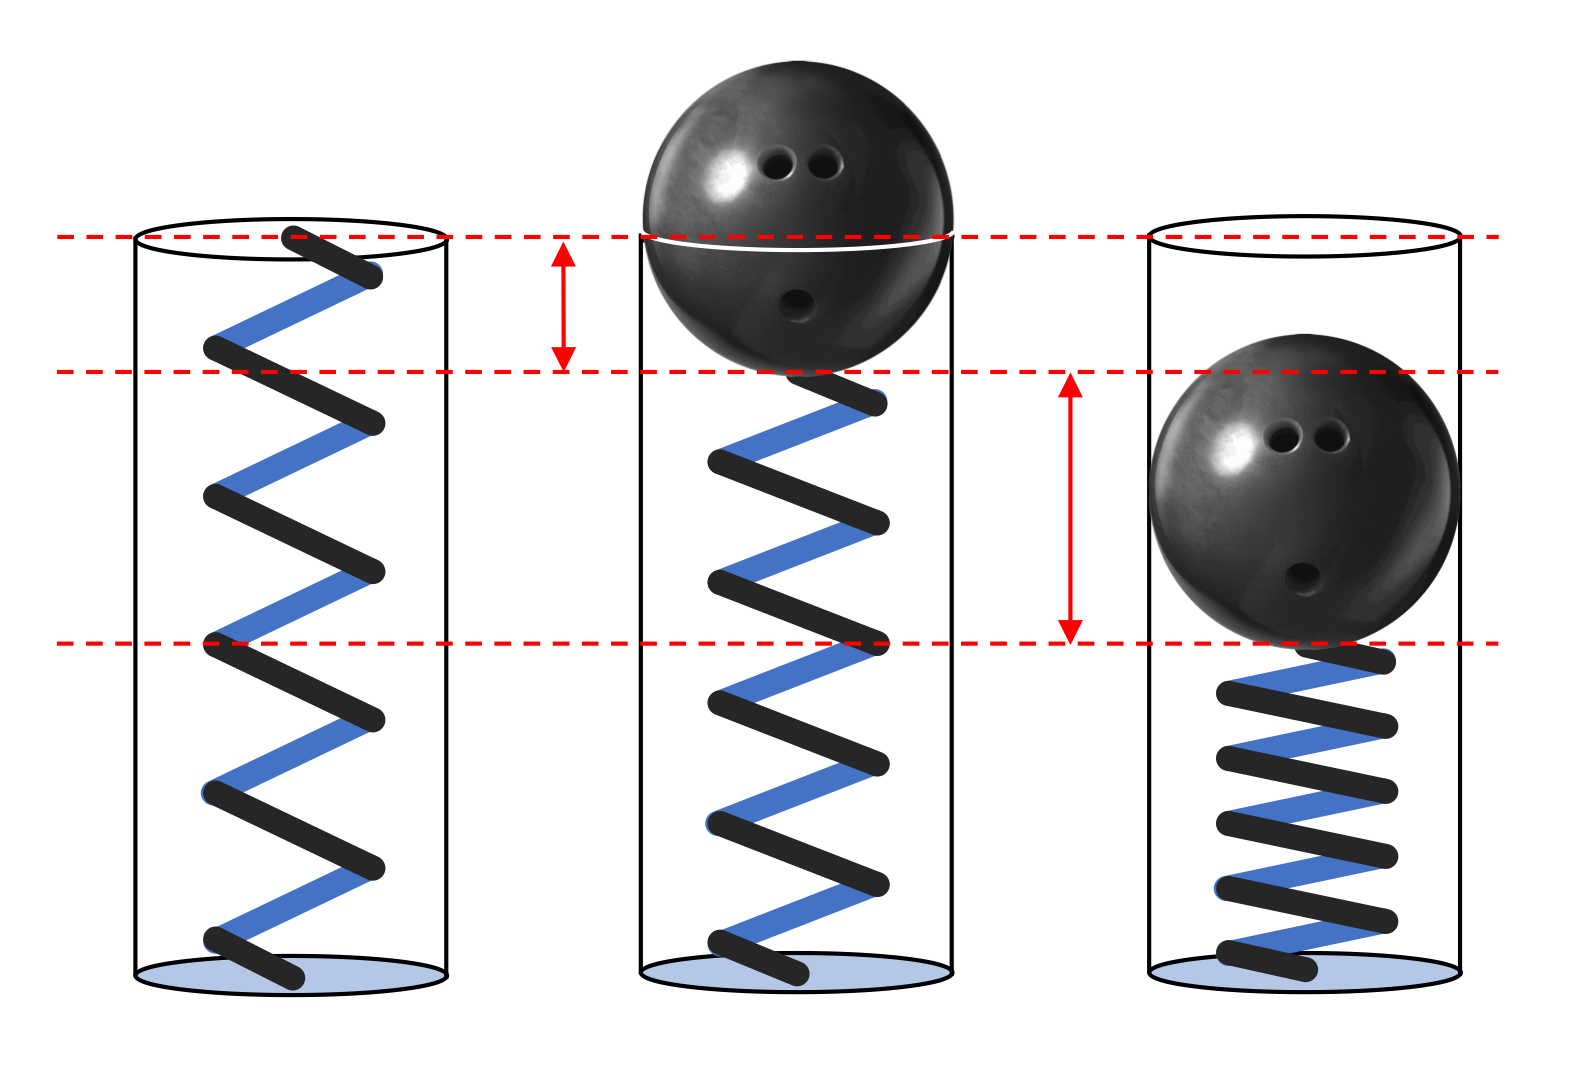
\includegraphics[width=0.6\textwidth]{Images/Kapittel3:Arbeid&Energi/cannonball_launcher.png}
    \caption{Fjærkaon i tyngdefelt}
    \label{fig:Fjær_i_tyngdefelt}
    \end{figure}
    
\exm{Kollisjon mellom legeme og fjær}{
Et legeme med masse \(100 \, \text{g}\) glir fra ro nedover en friksjonsfri bane og kolliderer med en elastisk fjær med fjærkonstanten \(k = 300 \, \text{N/m}\). Startpunktet for legemet er \(60 \, \text{cm}\) over den horisontale delen av banen. Vi skal først finne farten til legemet idet det treffer fjæren, og deretter finne hvor langt fjæren blir maksimalt presset inn under kollisjonen.

\textbf{Del a: Bestem farten til legemet idet det kolliderer med fjæren} \\
\textit{Metode:} \\
Vi bruker bevaring av mekanisk energi. I startposisjonen har legemet kun potensiell energi, og i det øyeblikket det treffer fjæren er all denne potensielle energien omformet til kinetisk energi (friksjon neglisjeres):
\[
E_p = E_k
\]
Ved bevaring av energi får vi:
\[
mgh = \frac{1}{2} m v^2
\]
Vi stryker massen \( m \) fra begge sider av likningen:
\[
gh = \frac{1}{2} v^2
\]
Løser for hastigheten \( v \):
\[
v = \sqrt{2gh}
\]
Setter inn verdiene \( g = 9.8 \, \text{m/s}^2 \) og \( h = 0.60 \, \text{m} \):
\[
v = \sqrt{2 \cdot 9.8 \, \text{m/s}^2 \cdot 0.60 \, \text{m}} = \sqrt{11.76} \approx \doubleunderline{ 3.43 \, \text{m/s}}
\]
Legemet har en hastighet på \( 3.43 \, \text{m/s} \) idet det treffer fjæren.

\vspace{20pt}  % 

\textbf{Del b: Hvor langt blir fjæren maksimalt presset inn?} \\
\textit{Metode:} \\
Nå overføres all den kinetiske energien fra legemet til fjæren, som blir maksimalt komprimert. Energien som lagres i den komprimerte fjæren er gitt ved elastisk potensiell energi:
\[
E_{\text{fjær}} = \frac{1}{2} k x^2
\]
Siden all den kinetiske energien omformes til elastisk potensiell energi ved maksimal kompresjon, setter vi \( E_k = E_{\text{fjær}} \):
\[
\frac{1}{2} m v^2 = \frac{1}{2} k x^2
\]
Vi kan stryke \( \frac{1}{2} \) fra begge sider:
\[
m v^2 = k x^2
\]
Løs for \( x \), som er maksimal kompresjon av fjæren:
\[
x = \sqrt{\frac{m v^2}{k}}
\]
Sett inn verdiene \( m = 0.1 \, \text{kg} \), \( v = 3.43 \, \text{m/s} \), og \( k = 300 \, \text{N/m} \):
\[
x = \sqrt{\frac{0.1 \, \text{kg} \cdot (3.43 \, \text{m/s})^2}{300 \, \text{N/m}}} = \sqrt{\frac{1.176}{300}} = \sqrt{0.00392} \approx \doubleunderline{0.063 \, \text{m}}
\]
Fjæren blir maksimalt komprimert med \( 6.3 \, \text{cm} \) under kollisjonen.
}

\begin{figure}[ht!]
    \centering
    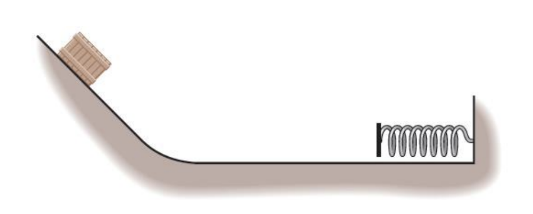
\includegraphics[width=0.9\textwidth]{Images/Kapittel3:Arbeid&Energi/Boksglir.png}
    \caption{Kollisjon mellom legme og fjær}
    \label{fig:Kollisjon}
    \end{figure}

\section{Effekt}
Effekt \( P \) er et mål på hvor raskt energi omformes eller utføres arbeid. Den defineres som mengden energi som overføres eller arbeidet som utføres per tidsenhet.

\defn{Effekt som arbeid per tidsenhet}{
    Effekt \( P \) kan uttrykkes som:
    \begin{align}
        P = \frac{W}{t}
    \end{align}
    hvor \( W \) er arbeidet eller energien som overføres, og \( t \) er tiden det tar.
}

Enheten for effekt er watt (W), der \( 1 \, \text{W} = 1 \, \text{J/s} \). Dette betyr at én watt tilsvarer at én joule energi overføres hvert sekund.

Effekt kan også uttrykkes i sammenheng med kraft og hastighet. Hvis en konstant kraft \( F \) virker på et objekt som beveger seg med en hastighet \( v \), kan effekten skrives som:

\defn{Effekt som kraft ganger hastighet}{
    Når en konstant kraft virker på et objekt i bevegelse, er effekten gitt ved:
    \begin{align}
        P = F \cdot v
    \end{align}
    hvor \( F \) er kraften som virker på objektet, og \( v \) er hastigheten.
}

Denne formelen viser at jo større kraft eller hastighet, desto mer arbeid utføres per tidsenhet, og dermed større effekt.


\section{Bevegelsesmengde}

Har du noen gang lurt på hvordan en rakett kan bevege seg i tomt rom, der det ikke finnes luft eller andre objekter å skyve fra? Svaret ligger i prinsippet om bevegelsesmengde. Selv om det ikke finnes noe å dytte mot i rommet, kan en rakett likevel akselerere ved å skyve ut gass med høy hastighet i motsatt retning. Dette skjer på grunn av bevaring av bevegelsesmengde.

Bevegelsesmengde, også kalt impulsmengde, er et mål på hvor mye bevegelse et objekt har, og det avhenger av både objektets masse og hastighet.

\defn{Bevegelsesmengde}{
    Bevegelsesmengden \( \vec{p} \) til et objekt er definert som:
    \begin{align}
        \vec{p} = m \cdot \vec{v}
    \end{align}
    hvor \( m \) er massen til objektet, og \( \vec{v} \) er objektets hastighet.
}

Bevegelsesmengden er en vektor, noe som betyr at den har både størrelse og retning. Større masse eller høyere hastighet gir mer bevegelsesmengde. For eksempel, en lastebil i bevegelse har mer bevegelsesmengde enn en sykkel i bevegelse, selv om de har samme hastighet, fordi lastebilen har mye større masse.

I lukkede systemer, der ingen ytre krefter virker, er bevegelsesmengden bevart. Dette prinsippet, kalt bevaringsloven, er grunnen til at en rakett kan bevege seg i rommet. Når raketten skyver gassen ut bakover, får gassen en bevegelsesmengde i én retning, og raketten får en like stor, men motsatt bevegelsesmengde, som fører til at raketten beveger seg fremover.

\defn{Bevaring av bevegelsesmengde}{
    I et lukket system, der ingen ytre krefter virker, er den totale bevegelsesmengden bevart. Dette kan uttrykkes som:
    \begin{align}
        \vec{p}_{\text{før}} = \vec{p}_{\text{etter}}
    \end{align}
    hvor \( \vec{p}_{\text{før}} \) er den totale bevegelsesmengden til systemet før en hendelse, og \( \vec{p}_{\text{etter}} \) er den totale bevegelsesmengden etter hendelsen. 
}

\subsection{Elastisk støt}

Et elastisk støt er en kollisjon der både den totale bevegelsesmengden og den totale kinetiske energien er bevart. I slike kollisjoner ``sprettes''
 objektene fra hverandre uten å miste energi til deformasjon eller varme, noe som betyr at den kinetiske energien er den samme før og etter kollisjonen.

I et elastisk støt mellom to objekter, gjelder både bevaring av bevegelsesmengde og bevaring av kinetisk energi:

\defn{Bevaring av bevegelsesmengde}{
    I et elastisk støt er bevegelsesmengden bevart:
    \begin{align}
        m_1 v_{1, \text{før}} + m_2 v_{2, \text{før}} = m_1 v_{1, \text{etter}} + m_2 v_{2, \text{etter}}
    \end{align}
    hvor \( m_1 \) og \( m_2 \) er massene til de to objektene, og \( v_{1, \text{før}} \), \( v_{2, \text{før}} \), \( v_{1, \text{etter}} \) og \( v_{2, \text{etter}} \) er hastighetene til objektene før og etter kollisjonen.
}

\defn{Bevaring av kinetisk Energi}{
    I et elastisk støt er også den kinetiske energien bevart:
    \begin{align}
        \frac{1}{2} m_1 v_{1, \text{før}}^2 + \frac{1}{2} m_2 v_{2, \text{før}}^2 = \frac{1}{2} m_1 v_{1, \text{etter}}^2 + \frac{1}{2} m_2 v_{2, \text{etter}}^2
    \end{align}
    Dette betyr at den totale kinetiske energien før kollisjonen er lik den totale kinetiske energien etter kollisjonen.
}

Et klassisk eksempel på elastisk støt er to biljardkuler som kolliderer. Når de treffer hverandre, blir ingen energi tapt til varme eller deformasjon, så de spretter fra hverandre, og den totale bevegelsesmengden og kinetiske energien forblir den samme.

\begin{figure}[ht!]
    \centering
    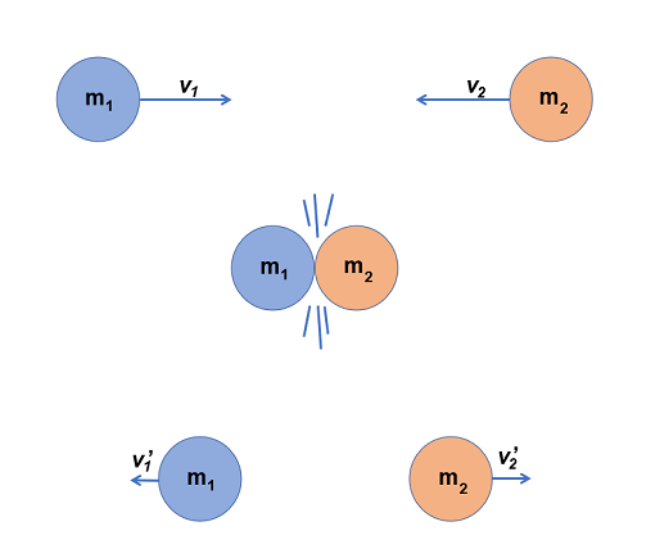
\includegraphics[width=0.7\textwidth]{Images/Kapittel3:Arbeid&Energi/Elastiskstøt1.png}
    \caption{Elastisk støt}
    \label{fig:Eks: Elastisk støt}
    \end{figure}

Et klassisk eksempel på bevaring av bevegelsesmengde og kinetisk energi finner vi i et eksperiment kjent som Newtons pendel. Dette består av flere kuler som henger på snorer og er i kontakt med hverandre. Når du løfter én av kulene fra den ene enden og slipper den, vil den kollidere med kulen ved siden av, som overfører bevegelsesmengden gjennom alle kulene. 

På grunn av bevaringen av bevegelsesmengde og kinetisk energi, vil den siste kulen i den andre enden ``skytes`` opp med omtrent samme hastighet som den første kulen ble sluppet. Resten av kulene forblir i ro etter kollisjonen.

Dette skjer fordi i et elastisk støt mellom objektene, bevares både den totale bevegelsesmengden og den totale kinetiske energien i systemet. I Newtons pendel ser vi disse prinsippene tydelig:
\[
m v_{\text{før}} = m v_{\text{etter}}
\]
\[
\frac{1}{2} m v_{\text{før}}^2 = \frac{1}{2} m v_{\text{etter}}^2
\]
Dette viser at kulene overfører bevegelsesmengde og energi fra den ene enden av pendelen til den andre uten at energi går tapt i prosessen.\\

I Newtons pendel skjer det elastiske kollisjoner mellom kulene. I en elastisk kollisjon bevares både bevegelsesmengden og den kinetiske energien, slik at ingen energi går tapt til varme eller deformasjon. Når én kule slippes, overføres bevegelsesmengden og energien gjennom de midterste kulene til den siste kulen i rekken, som "spretter" opp med samme hastighet som den første. 

\begin{figure}[H]
    \centering
    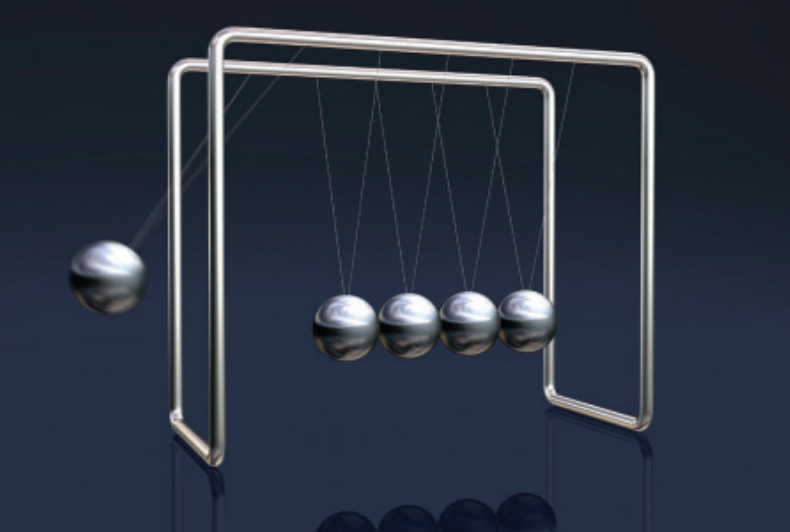
\includegraphics[width=0.6\textwidth]{Images/Kapittel3:Arbeid&Energi/Newtons pendel.png}
    \caption{Newtons pendel}
    \label{fig:Eks: Newtons pendel}
    \end{figure}


\exm{Elastisk kollisjon mellom to like vogner}{
En vogn med masse \( m = 2.0 \, \text{kg} \) og fart \( v_1 = 3.0 \, \text{m/s} \) krasjer inn i en annen vogn med samme masse \( m = 2.0 \, \text{kg} \) som står stille (\( u = 0 \)) på et friksjonsfritt underlag. Det er ingen ytre krefter som virker på systemet (vogn 1 + vogn 2), og det utføres ikke arbeid på systemet under kollisjonen. Vi skal finne hastighetene til begge vognene etter kollisjonen.

\textit{Løsning:} \\
Siden det er en elastisk kollisjon, er både bevegelsesmengden og den kinetiske energien bevart.

\textbf{Bevaring av Bevegelsesmengde:} \\
Før kollisjonen har bare vogn 1 bevegelsesmengde, siden vogn 2 står stille:
\[
p_{\text{før}} = m v_1
\]
Etter kollisjonen får vi at bevegelsesmengden fordeler seg mellom vogn 1 (med hastighet \( v_2 \)) og vogn 2 (med hastighet \( u \)):
\[
p_{\text{etter}} = m v_2 + m u
\]
Siden bevegelsesmengden er bevart, har vi:
\[
m v_1 = m v_2 + m u
\]
Vi kan forkorte \( m \) fra begge sider:
\[
v_1 = v_2 + u
\]

\textbf{Bevaring av kinetisk Energi:} \\
I en elastisk kollisjon bevares også den kinetiske energien. Kinetisk energi før kollisjonen er bare fra vogn 1:
\[
E_{\text{før}} = \frac{1}{2} m v_1^2
\]
Etter kollisjonen er den kinetiske energien fordelt mellom begge vognene:
\[
E_{\text{etter}} = \frac{1}{2} m v_2^2 + \frac{1}{2} m u^2
\]
Siden kinetisk energi er bevart, har vi:
\[
\frac{1}{2} m v_1^2 = \frac{1}{2} m v_2^2 + \frac{1}{2} m u^2
\]
Igjen kan vi forkorte \( \frac{1}{2} m \) fra begge sider:
\[
v_1^2 = v_2^2 + u^2
\]

\textbf{Løsning for hastighetene \( v_2 \) og \( u \):} \\
Vi har nå to ligninger:
1. \( v_1 = v_2 + u \)
2. \( v_1^2 = v_2^2 + u^2 \)

Ved å substituere \( u = v_1 - v_2 \) fra den første ligningen inn i den andre ligningen, får vi:
\[
v_1^2 = v_2^2 + (v_1 - v_2)^2
\]
Utvid \( (v_1 - v_2)^2 \):
\[
v_1^2 = v_2^2 + v_1^2 - 2 v_1 v_2 + v_2^2
\]
Forenkle ved å samle ledd:
\[
v_1^2 = 2v_2^2 - 2v_1 v_2 + v_1^2
\]
Trekk \( v_1^2 \) fra begge sider:
\[
0 = 2v_2^2 - 2v_1 v_2
\]
Del begge sider på 2:
\[
0 = v_2(v_2 - v_1)
\]
Dette gir to mulige løsninger: enten \( v_2 = 0 \) eller \( v_2 = v_1 \). Men siden vogn 1 overfører all sin bevegelse til vogn 2 (den elastiske kollisjonen), må \( v_2 = 0 \). Dermed har vi:
\[
v_2 = 0 \quad \text{og} \quad u = v_1 = 3.0 \, \text{m/s}
\]

Etter kollisjonen står vogn 1 stille (\( v_2 = 0 \)), og vogn 2 beveger seg med en fart på \( u = 3.0 \, \text{m/s} \).
}

\newpage

\subsection{Uelastisk Støt}

I et uelastisk støt er ikke den kinetiske energien bevart. Dette betyr at noe av den kinetiske energien blir omformet til andre energiformer, som varme, lyd eller deformasjon. Bevegelsesmengden er fortsatt bevart, men den totale kinetiske energien før og etter kollisjonen vil ikke være den samme.

Et eksempel på et uelastisk støt er når to biler kolliderer og "henger sammen" etter kollisjonen. I slike tilfeller mister systemet en del av sin kinetiske energi, som går over til deformasjon av bilene, lyd og varme.


\defn{Bevaring av bevegelsesmengde ved uelastisk støt}{
    I et uelastisk støt, der to objekter henger sammen etter kollisjonen, uttrykkes bevaringen av bevegelsesmengde som:
    \begin{align}
        m_1 v_{1, \text{før}} + m_2 v_{2, \text{før}} = (m_1 + m_2) v_{\text{etter}}
    \end{align}
    hvor \( m_1 \) og \( m_2 \) er massene til objektene, \( v_{1, \text{før}} \) og \( v_{2, \text{før}} \) er hastighetene før kollisjonen, og \( v_{\text{etter}} \) er den felles hastigheten etter kollisjonen dersom objektene henger sammen.
}


I et uelastisk støt er kinetisk energi tapt, men bevegelsesmengden er alltid bevart.
\\

\begin{figure}[H]
    \centering
    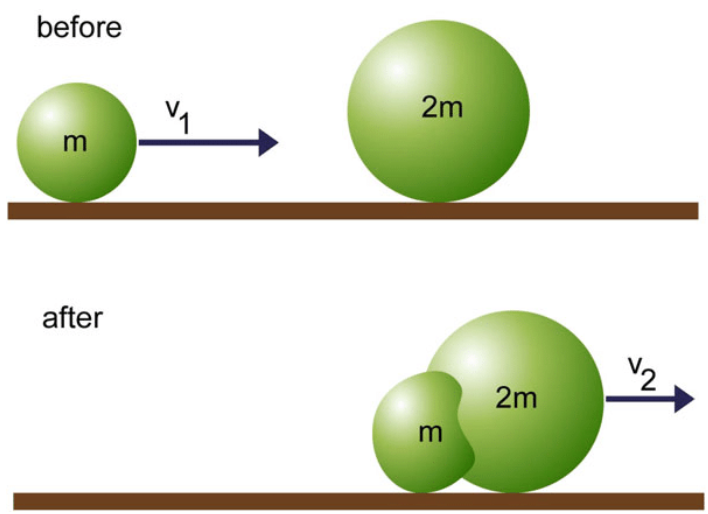
\includegraphics[width=0.6\textwidth]{Images/Kapittel3:Arbeid&Energi/Uleastisk1.png}
    \caption{Uelastisk støt}
    \label{fig:Eks: Uelastisk støt}
    \end{figure}

\exm{Uelastisk kollisjon mellom en ball og en vogn}{
En ball med masse \( m_{\text{ball}} = 0.5 \, \text{kg} \) kastes rett inn i en stillestående vogn med masse \( m_{\text{vogn}} = 2.0 \, \text{kg} \). Ballen har en hastighet på \( v_{\text{ball}} = 20 \, \text{m/s} \) idet den treffer vognen. Etter sammenstøtet beveger ballen og vognen seg sammen med samme hastighet. Vi skal finne denne felles hastigheten \( v_{\text{etter}} \) for ball + vogn etter kollisjonen.

\textit{Løsning:} \\
Dette er et eksempel på et uelastisk støt, der ballen og vognen henger sammen etter kollisjonen. Selv om den kinetiske energien ikke er bevart, er bevegelsesmengden bevart, siden det ikke er noen ytre krefter som virker på systemet.

\textbf{Bevaring av Bevegelsesmengde:} \\
Før kollisjonen har vi bare bevegelsesmengden til ballen, siden vognen står stille:
\[
p_{\text{før}} = m_{\text{ball}} \cdot v_{\text{ball}} + m_{\text{vogn}} \cdot 0 = m_{\text{ball}} \cdot v_{\text{ball}}
\]
Etter kollisjonen beveger ballen og vognen seg sammen med hastigheten \( v_{\text{etter}} \):
\[
p_{\text{etter}} = (m_{\text{ball}} + m_{\text{vogn}}) \cdot v_{\text{etter}}
\]
Siden bevegelsesmengden er bevart, har vi:
\[
m_{\text{ball}} \cdot v_{\text{ball}} = (m_{\text{ball}} + m_{\text{vogn}}) \cdot v_{\text{etter}}
\]
Løs for \( v_{\text{etter}} \):
\[
v_{\text{etter}} = \frac{m_{\text{ball}} \cdot v_{\text{ball}}}{m_{\text{ball}} + m_{\text{vogn}}}
\]
Sett inn verdiene \( m_{\text{ball}} = 0.5 \, \text{kg} \), \( v_{\text{ball}} = 20 \, \text{m/s} \), og \( m_{\text{vogn}} = 2.0 \, \text{kg} \):
\[
v_{\text{etter}} = \frac{0.5 \cdot 20}{0.5 + 2.0} = \frac{10}{2.5} = 4 \, \text{m/s}
\]
Etter kollisjonen beveger ballen og vognen seg sammen med en felles hastighet på \( v_{\text{etter}} = 4 \, \text{m/s} \).
}

